\setchapterpreamble[u]{%
    \dictum[C. Lloyd como Dr. Emmet Brown en \textit{Regreso al Futuro}] {\textquote{It works, it works! I finally invented something that works!}}
}
\chapter{Resultados de las simulaciones conductuales}

\section{Simulación conductual de la NoC}
\label{sec:resNoC}

En esta sección se analizan los datos generados por la simulación de comportamiento del RTL de la NoC de $3\times3$ y 16 bits por flit, explicada en la subsección \ref{subsec:rtl_simulacion}. Para ello se han usado herramientas de análisis de datos como Pandas y Numpy, generando las gráficas con Matplotlib. En la carpeta \texttt{data} del repositorio del proyecto\footnote{\url{https://github.com/ogarnica/TFG2021-22_RISC-V_NoC/tree/main/data}} pueden encontrarse los datos generados por la simulación y el Jupyter Notebook para el procesado de estos.

Durante la prueba de la red se emiten paquetes con información generada aleatoriamente, de un tamaño también aleatorio de entre 1 y 160 bits (2 a 12 flits, contando la cabecera) siguiendo en ambos casos distribuciones uniformes. Por lo tanto, el tamaño medio de los paquetes es de $6.5$ flits. Para simular distintas condiciones de red, la cantidad de paquetes en la NoC aumenta de manera lineal conforme avanza el tiempo de la simulación.

Las simulaciones, tanto conductuales como post-síntesis (teniendo en cuenta los retardos de las puertas y conexiones), han sido satisfactorias, sin producirse ningún tipo de bloqueo (véase \ref{subsec:routing-problems} \nameref{subsec:routing-problems}), ni pérdida de paquetes.

En total, en la NoC se han emitido $31009$ paquetes a lo largo de más de $100000$ ciclos, enviando un total de 2.5 megabits de datos haciendo uso de $171997$ flits.

\subsection{Detección de problemas}

La probabilidad de que se presenten problemas en una red aumenta cuanto mayor sea la carga de la red, pues más recursos estarán bloqueados al mismo tiempo y más probable es que se intente acceder a un recurso bloqueado. Por ello, se han hecho pruebas aumentando la carga de la red de manera lineal. El único problema detectado en nuestra red es cierto grado de \textit{starvation} cuando la carga es muy elevada, pero nunca superando los 16 ciclos de espera. La figura~\ref{fig:starvationWait} muestra que hay una fuerte correlación entre la ocupación de la red y el tiempo de espera, llegando a su máximo a partir del ciclo 80000, en el que hay 11 paquetes haciendo uso de la red y el tiempo de espera medio es de 15 ciclos. Para calcular el número de paquetes en la red se han restado la suma cumulativa del número de paquetes salientes y la suma cumulativa del número de paquetes que han establecido una conexión, por lo que no se cuentan las emisiones en las que aún se está estableciendo una conexión, a pesar de que también bloquean recursos.

\begin{figure}[h]
    \centering
    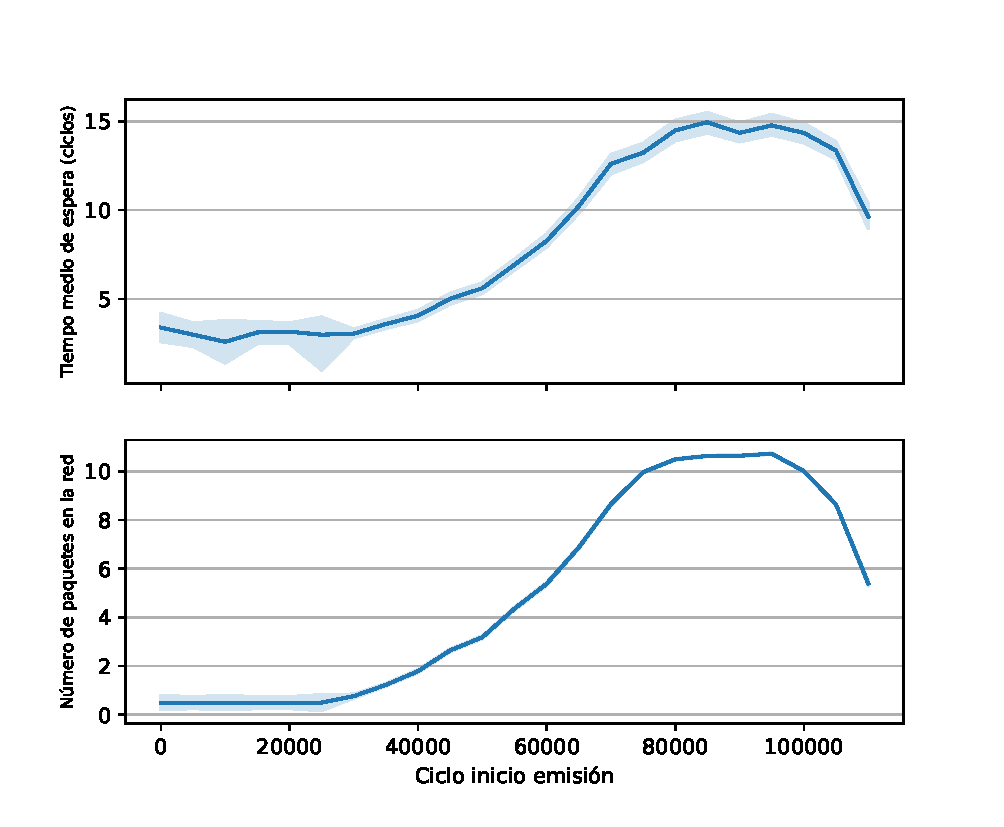
\includegraphics[width=.9\linewidth]{images/plots/wait_packets.pdf}
    \caption[Tiempo de espera hasta inicio de emisión y carga de la red.]{Tiempo de espera medio hasta inicio de emisión y carga de la red en una red 3x3 (el sombreado indica la desviación típica de la media). La carga de la red aumenta desde el ciclo 30000 de manera linear hasta saturar la red.}
    \label{fig:starvationWait}
\end{figure}

% \tdinquiry[inline, caption={Cosas por hacer simulación}]{
% \begin{itemize}
%     \item Creo que quedaría bien poner la tasa de bits de la red a lo largo del tiempo en bits por ciclo si es posible, pero solo si da tiempo. 
%     \item ¿Alguna idea?
% \end{itemize}
% }

\section{Simulación conductual del SweRV-EL2}
Para verificar el procesador, ha de utilizarse un simulador para ejecutar un modelo del diseño RTL, cargando en la memoria del procesador cualquier programa escrito en C o ensamblador.

Con objeto de facilitar esta tarea, una de las herramientas incluidas en el proyecto original del SweRV-EL2 es un fichero \textit{Makefile}, que compila el programa a cargar en la memoria y simula el \textit{core}, permitiendo seleccionar el simulador a utilizar.

Se ha modificado la parte del \textit{Makefile} para que, cuando se seleccione \textit{QuestaSim} como simulador, se incluyan también los ficheros de la NoC. También ha sido necesario modificar el \textit{testbench} (fichero SystemVerilog encargado de definir los estímulos de entrada y verificar las salidas), añadiendo únicamente el nuevo reloj para la NoC de la EXU.

Durante el desarrollo, para comprobar el funcionamiento del procesador tras realizar pequeñas modificaciones en el diseño, se ha ejecutado un pequeño programa que imprime las palabras ``Hello World'' en la salida estándar del simulador (figura \ref{fig:sim_hw}). Si dicho test termina satisfactoriamente, se procede a ejecutar \textit{CoreMark}, un \textit{benchmark} diseñado para probar la funcionalidad de un core \cite{EEMBCCoreMark}, ejecutando todo tipo de instrucciones. En la figura \ref{fig:sim_cmark} se presentan los resultados de dicho benchmark.

Observando los registros de ejecución generados en el fichero \textit{exec.log}, puede comprobarse que se ejecutan instrucciones de multiplicación y de división sin problemas, por lo que la implementación de la NoC ha sido satisfactoria.

\begin{figure}[hp]
    \centering
    \begin{minted}[fontsize=\scriptsize, bgcolor=lightgray!20]{console}
# run -all
# ----------------------------------
# Hello World from SweRV EL2 @WDC !!
# ----------------------------------
# TEST_PASSED
#
# Finished : minstret = 437, mcycle = 922
# See "exec.log" for execution trace with register updates..
#
# ** Note: $finish    : E:/TFG/TFG2021-22_RISC-V_NoC/Cores-SweRV-EL2/testbench/tb_top.sv(343)
#    Time: 9280 ns  Iteration: 1  Instance: /tb_top
# End time: 16:49:55 on May 29,2022, Elapsed time: 0:00:13
# Errors: 0, Warnings: 1375
    \end{minted}
    \captionof{figure}{Resultados de la simulación del programa \textit{hello\_world}.}
    \label{fig:sim_hw}
\end{figure}

\begin{figure}[hp]
    \centering
    \begin{minted}[fontsize=\scriptsize, bgcolor=lightgray!20]{console}
# run -all
# 2K performance run parameters for coremark.
# CoreMark Size    : 666
# Total ticks      : 416012
# Total time (secs): 416
# Iterat/Sec/MHz   : 2.57
# Iterations       : 1
# Compiler version : GCC9.2.0
# Compiler flags   : -g -O3 -funroll-all-loops
# Memory location  : STATIC
# seedcrc          : 0xe9f5
# [0]crclist       : 0xe714
# [0]crcmatrix     : 0x1fd7
# [0]crcstate      : 0x8e3a
# [0]crcfinal      : 0xe714
# Correct operation validated. See readme.txt for run and reporting rules.
# TEST_PASSED
#
# Finished : minstret = 304107, mcycle = 440127
# See "exec.log" for execution trace with register updates..
#
# ** Note: $finish    : E:/TFG/TFG2021-22_RISC-V_NoC/Cores-SweRV-EL2/testbench/tb_top.sv(343)
#    Time: 4401330 ns  Iteration: 1  Instance: /tb_top
# End time: 16:44:17 on May 29,2022, Elapsed time: 0:01:55
# Errors: 0, Warnings: 1375
    \end{minted}
    \captionof{figure}{Resultados de la simulación del programa \textit{Coremark}.}
    \label{fig:sim_cmark}
\end{figure}
